\documentclass[11pt,a4paper]{article}
\usepackage[textwidth=37em,vmargin=30mm]{geometry}
\usepackage{calc,xunicode,amsmath,amssymb,paralist,enumitem,tabu,booktabs,datetime2,xeCJK,xeCJKfntef,listings}
\usepackage{tocloft,fancyhdr,tcolorbox,xcolor,graphicx,eso-pic,xltxtra,xelatexemoji}

\usepackage[hidelinks]{hyperref}
\hypersetup{
    colorlinks=false,
    pdfpagemode=FullScreen,
    pdftitle={Web Digest - 2023-01-11}
}

\setdefaultleftmargin{2em}{2em}{1em}{1em}{1em}{1em}

\usepackage{xeCJK,xeCJKfntef}
\newcommand{\myvphantom}[0]{\vphantom{QWERTYUIOPASDFGHJKLZXCVBNMqwertyuiopasdfghjklzxcvbnm1234567890ςρθδφγηξλζχψβμ\"A}}
\xeCJKsetup{PunctStyle=plain,RubberPunctSkip=false,CJKglue=\myvphantom\hskip 0pt plus 0.1em minus 0.05em,CJKecglue=\myvphantom\hskip 0.22em plus 200pt}
\XeTeXlinebreaklocale "zh"
\XeTeXlinebreakskip = 0pt


\setmainfont{Brygada 1918}
\setromanfont{Brygada 1918}
\setsansfont{IBM Plex Sans}
\setmonofont{JetBrains Mono NL}
\setCJKmainfont{Noto Serif CJK SC}
\setCJKromanfont{Noto Serif CJK SC}
\setCJKsansfont{Noto Sans CJK SC}
\setCJKmonofont{Noto Sans CJK SC}

\setlength{\parindent}{0pt}
\setlength{\parskip}{8pt}
\linespread{1.15}

\lstset{
	basicstyle=\ttfamily\footnotesize,
	numbersep=5pt,
	backgroundcolor=\color{black!5},
	showspaces=false,
	showstringspaces=false,
	showtabs=false,
	tabsize=2,
	captionpos=b,
	breaklines=true,
	breakatwhitespace=true,
	breakautoindent=true,
	linewidth=\textwidth
}






\newcommand{\coverpic}[2]{
    % argv: itemurl, authorname
    Cover photo by #2~~(\href{#1}{#1})
}
\newcommand{\makeheader}[0]{
    \begin{titlepage}
        % \newgeometry{hmargin=15mm,tmargin=21mm,bmargin=12mm}
        \begin{center}
            
            \rmfamily\scshape
            \fontspec{BaskervilleF}
            \fontspec{Old Standard}
            \fontsize{59pt}{70pt}\selectfont
            WEB\hfill DIGEST
            
            \vfill
            % \vskip 30pt
            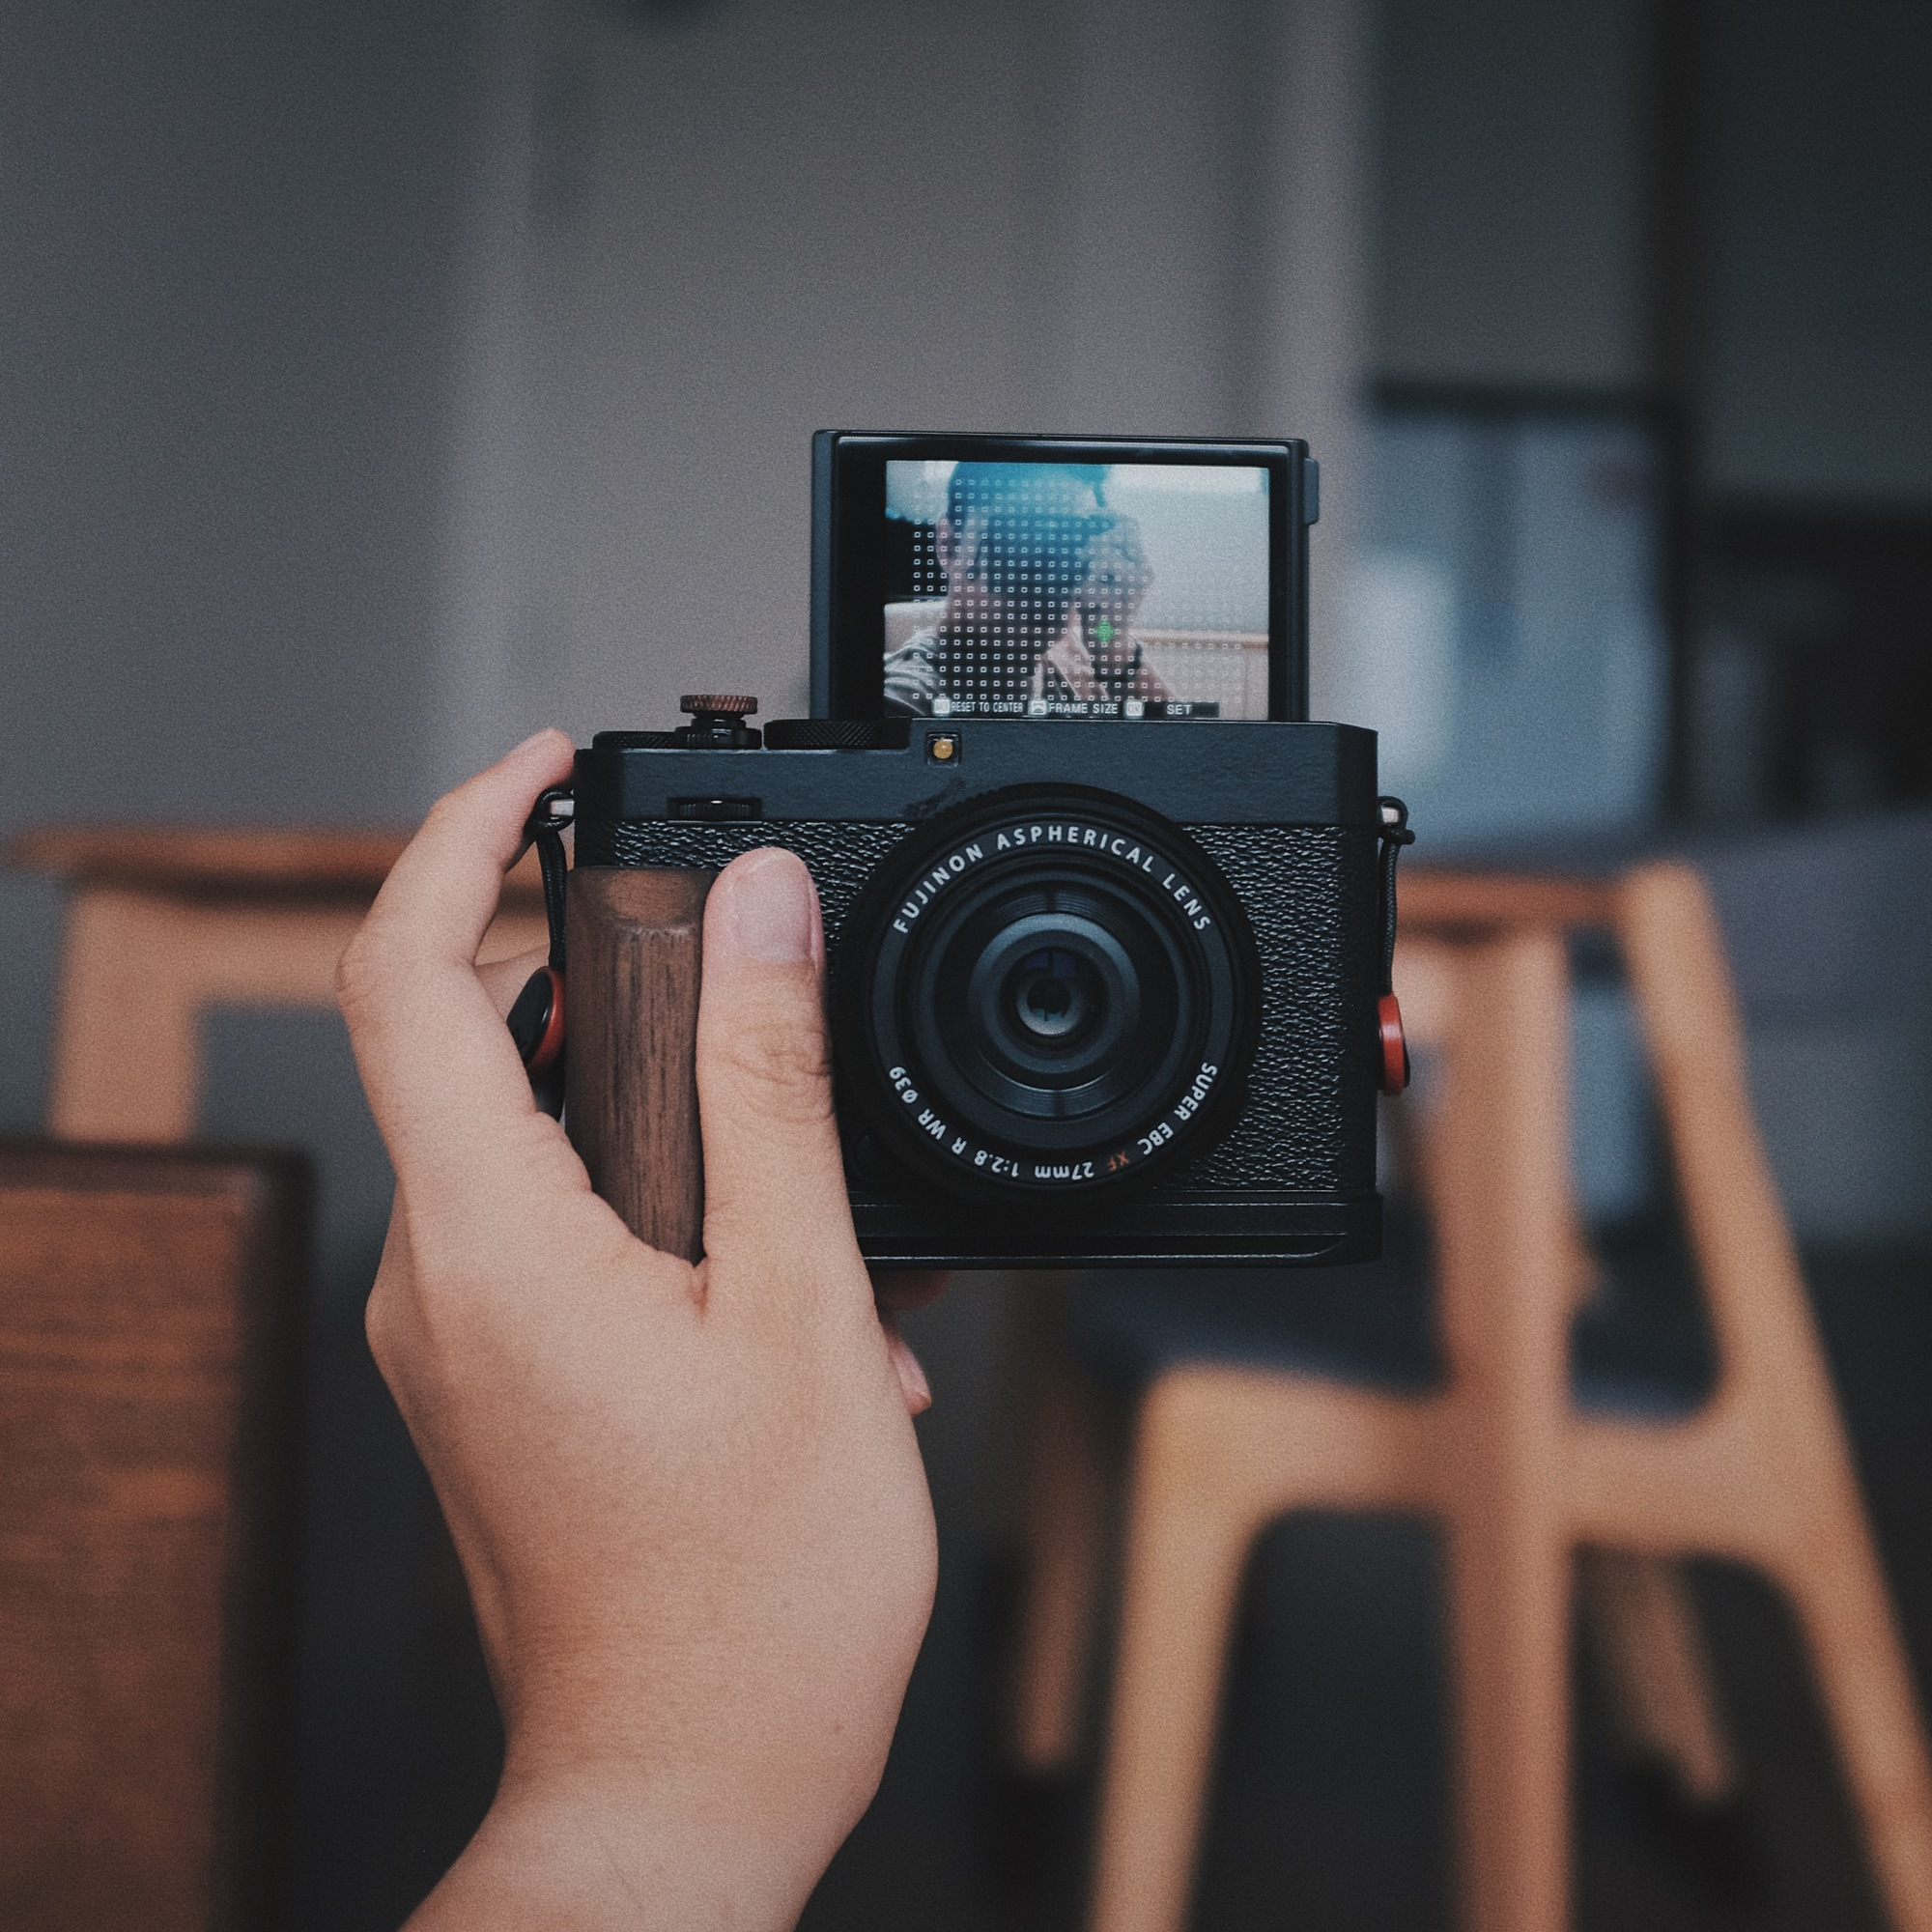
\includegraphics[width=\linewidth]{webdb/2023/20230111/final/coverpic-prod.jpg}\par
            % \vskip 30pt
            \vfill

            \normalsize\rmfamily\scshape
            \copyright{} The Web Digest Project \hfill\large 2023-01-11
        \end{center}
    \end{titlepage}
    % \restoregeometry
}
\newcommand{\simplehref}[1]{%
    \textcolor{blue!80!green}{\href{#1}{#1}}%
}
\renewcommand{\contentsname}{\center\Huge\sffamily\bfseries Contents\par\vskip 20pt}
\newcounter{ipartcounter}
\setcounter{ipartcounter}{0}
\newcommand{\ipart}[1]{
    % \vskip 20pt
    \clearpage
    \stepcounter{ipartcounter}
    \phantomsection
    \addcontentsline{toc}{section}{#1}
    \begin{center}
        \Huge
        \sffamily\bfseries
        #1
    \end{center}
    \vskip 20pt
}
\newcommand{\entrytitlefont}[0]{\Large\sffamily\bfseries}
\newcommand{\entryitemGeneric}[2]{
    % argv: title, url
    \parbox{\linewidth}{
        \entrytitlefont#1\par\vskip 5pt
        \footnotesize\ttfamily\mdseries
        \simplehref{#2}\par
    }\vskip 11pt
}
\newcommand{\entryitemGithub}[3]{
    % argv: title, url, desc
    \parbox{\linewidth}{
        \entrytitlefont#1\par\vskip 5pt
        \footnotesize\ttfamily\mdseries
        \simplehref{#2}\par\vskip 5pt
        \small\rmfamily\mdseries#3
    }\vskip 11pt
}
\newcommand{\entryitemAp}[3]{
    % argv: title, url, desc
    \parbox{\linewidth}{
        \entrytitlefont#1\par\vskip 5pt
        \footnotesize\ttfamily\mdseries
        \simplehref{#2}\par\vskip 5pt
        \small\rmfamily\mdseries#3
    }\vskip 11pt
}
\newcommand{\entryitemHackernews}[3]{
    % argv: title, hnurl, rawurl
    \parbox{\linewidth}{
        \entrytitlefont#1\par\vskip 5pt
        \footnotesize\ttfamily\mdseries
        \simplehref{#3}\par
        \textcolor{black!50}{\href{#2}{#2}}\par
    }\vskip 11pt
}






\begin{document}

\makeheader

\tableofcontents\clearpage


\ipart{Hacker News}
\entryitemHackernews{\hskip 0pt{}Pirate Weather: A free, open, and documented forecast API}{https://news.ycombinator.com/item?id=34329988}{https://pirateweather.net/}

\entryitemHackernews{\hskip 0pt{}Ask HN: What do you talk about in 1-on-1s with your managers?}{https://news.ycombinator.com/item?id=34329351}{https://news.ycombinator.com/item?id=34329351}

\entryitemHackernews{\hskip 0pt{}X Window System Basics (2014)}{https://news.ycombinator.com/item?id=34328777}{https://magcius.github.io/xplain/article/x-basics.html}

\entryitemHackernews{\hskip 0pt{}Theory-building and why employee churn is lethal to software companies}{https://news.ycombinator.com/item?id=34328069}{https://www.baldurbjarnason.com/2022/theory-building/}

\entryitemHackernews{\hskip 0pt{}Surveillance Footage of Tesla Crash on SF's Bay Bridge}{https://news.ycombinator.com/item?id=34327763}{https://theintercept.com/2023/01/10/tesla-crash-footage-autopilot/}

\entryitemHackernews{\hskip 0pt{}How Microsoft attempted to make the Xbox 360 dashboard load faster}{https://news.ycombinator.com/item?id=34327759}{https://eaton-works.com/2023/01/09/how-microsoft-attempted-to-make-the-xbox-360-dashboard-load-faster/}

\entryitemHackernews{\hskip 0pt{}Learn Lisp the Hard Way}{https://news.ycombinator.com/item?id=34326311}{https://llthw.common-lisp.dev/}

\entryitemHackernews{\hskip 0pt{}Fewer than 40\% of New Yorkers earn a living wage}{https://news.ycombinator.com/item?id=34326292}{https://news.cornell.edu/stories/2023/01/fewer-40-new-yorkers-earn-living-wage}

\entryitemHackernews{\hskip 0pt{}`Films are vulnerable': The battle to preserve Eastern Europe's analogue movies (2022)}{https://news.ycombinator.com/item?id=34325951}{https://www.calvertjournal.com/features/show/13454/films-are-vulnerable-the-battle-to-preserve-eastern-europes-films}

\entryitemHackernews{\hskip 0pt{}Tech companies are irrational pop cultures}{https://news.ycombinator.com/item?id=34325852}{https://softwarecrisis.dev/letters/tech-is-a-pop-culture/}

\entryitemHackernews{\hskip 0pt{}Taking over a Dead IoT Company}{https://news.ycombinator.com/item?id=34325695}{https://blog.kchung.co/taking-over-a-dead-iot-company/}

\entryitemHackernews{\hskip 0pt{}Microsoft in talks to acquire a 49\% stake in ChatGPT owner OpenAI}{https://news.ycombinator.com/item?id=34325217}{https://watcher.guru/news/microsoft-plans-to-acquire-a-49-stake-in-chatgpt-owner-openai}

\entryitemHackernews{\hskip 0pt{}Ask HN: I'm 40 and feel my mental ability declining. Programming seems harder.}{https://news.ycombinator.com/item?id=34324567}{https://news.ycombinator.com/item?id=34324567}

\entryitemHackernews{\hskip 0pt{}Tell HN: We Need Robots.txt but for AI}{https://news.ycombinator.com/item?id=34324208}{https://news.ycombinator.com/item?id=34324208}

\entryitemHackernews{\hskip 0pt{}Douglas Adams on Hypercard and new educational models}{https://news.ycombinator.com/item?id=34324169}{https://arbesman.substack.com/p/open-ended-software-as-human-beings}

\entryitemHackernews{\hskip 0pt{}It's not just what you eat, but the time of day you eat it}{https://news.ycombinator.com/item?id=34324120}{https://www.washingtonpost.com/wellness/2023/01/10/meal-timing-big-meals/}

\entryitemHackernews{\hskip 0pt{}Rackspace founder says it's `on trajectory of death.'}{https://news.ycombinator.com/item?id=34323674}{https://www.expressnews.com/business/article/Rackspace-Yoo-ransomware-attack-17703197.php}

\entryitemHackernews{\hskip 0pt{}UK: Excess deaths in 2022 among worst in 50 years}{https://news.ycombinator.com/item?id=34323469}{https://www.bbc.co.uk/news/health-64209221}

\entryitemHackernews{\hskip 0pt{}Coinbase cuts staff by a further 20\%}{https://news.ycombinator.com/item?id=34323336}{https://www.coinbase.com/blog/a-message-from-ceo-and-co-founder-brian-armstrong-to-coinbase-employees}

\entryitemHackernews{\hskip 0pt{}Faster PostgresSQL to BigQuery Transfers}{https://news.ycombinator.com/item?id=34323258}{https://tech.marksblogg.com/postgresql-to-bigquery.html}

\ipart{V2EX}
\entryitemGeneric{\hskip 0pt{}[设计师] 有偿重新设计 App 图标}{https://www.v2ex.com/t/908052}

\entryitemGeneric{\hskip 0pt{}[分享发现] Jane 这个名字也可以男生用}{https://www.v2ex.com/t/908051}

\entryitemGeneric{\hskip 0pt{}[问与答] 冬天还有好多蚊子不想挂蚊帐有什么招?}{https://www.v2ex.com/t/908050}

\entryitemGeneric{\hskip 0pt{}[汽车] 消费降级买个比亚迪可行?}{https://www.v2ex.com/t/908049}

\entryitemGeneric{\hskip 0pt{}[iOS] iOS App Store 今天推了这个神棍..}{https://www.v2ex.com/t/908048}

\entryitemGeneric{\hskip 0pt{}[程序员] 如何从理论上避免这类并行任务交错执行时的冲突问题}{https://www.v2ex.com/t/908047}

\entryitemGeneric{\hskip 0pt{}[Wikipedia] PC 使用维基百科为什么默认进入是移动版?}{https://www.v2ex.com/t/908046}

\entryitemGeneric{\hskip 0pt{}[分享发现] 微软的 Azure 似乎没有用自家的 ASP.NET Core 的前端框架}{https://www.v2ex.com/t/908045}

\entryitemGeneric{\hskip 0pt{}[问与答] 附近的工厂噪音问题如何匿名投诉?}{https://www.v2ex.com/t/908044}

\entryitemGeneric{\hskip 0pt{}[VPS] 有没有出水墨云 IPLC 沪美转发小流量的?}{https://www.v2ex.com/t/908042}

\entryitemGeneric{\hskip 0pt{}[Google] 谷歌搜索又被下毒}{https://www.v2ex.com/t/908041}

\entryitemGeneric{\hskip 0pt{}[macOS] 请问如何删除根目录下的"opt"文件夹}{https://www.v2ex.com/t/908040}

\entryitemGeneric{\hskip 0pt{}[Android] 一种新的 Magisk 安装方法,免 ROM 解包,不需要 TWRP,还有点 NTR}{https://www.v2ex.com/t/908038}

\entryitemGeneric{\hskip 0pt{}[Docker] 阿里云源 pull 下来的 Docker image 架构不正确}{https://www.v2ex.com/t/908037}

\entryitemGeneric{\hskip 0pt{}[Android] Google maps 无法定位}{https://www.v2ex.com/t/908036}

\entryitemGeneric{\hskip 0pt{}[程序员] ygc 一秒一次,一次停顿 15m 左右正常么}{https://www.v2ex.com/t/908035}

\entryitemGeneric{\hskip 0pt{}[程序员] windows 装 NAS 该用什么软件?}{https://www.v2ex.com/t/908034}

\entryitemGeneric{\hskip 0pt{}[iCloud] 土耳其 iCloud 支付问题}{https://www.v2ex.com/t/908033}

\entryitemGeneric{\hskip 0pt{}[酷工作] [远端] 招聘 ODOO 攻城狮}{https://www.v2ex.com/t/908032}

\entryitemGeneric{\hskip 0pt{}[AirPods] 突然发现 AirPods Pro 可以调整提示音音量了}{https://www.v2ex.com/t/908030}

\entryitemGeneric{\hskip 0pt{}[Apple] macos 这什么脑残 bug}{https://www.v2ex.com/t/908029}

\entryitemGeneric{\hskip 0pt{}[NAS] 寻求群晖 Synology 图书管理系统,可 Docker,已排除 Calibre-WebTaleBook,内详}{https://www.v2ex.com/t/908028}

\entryitemGeneric{\hskip 0pt{}[问与答] Chrome 历史里面这个时间是怎么算得 似乎不是时间戳}{https://www.v2ex.com/t/908027}

\entryitemGeneric{\hskip 0pt{}[分享创造] 分享最近开发的一个 Tableau 的开源替代项目}{https://www.v2ex.com/t/908026}

\entryitemGeneric{\hskip 0pt{}[Java] 请问 feign 只能通过硬编码指定 encoder, decoder 等配置吗?}{https://www.v2ex.com/t/908025}

\entryitemGeneric{\hskip 0pt{}[问与答] 才发现,语雀写作后,分享互联网是需要付费的,好尴尬}{https://www.v2ex.com/t/908024}

\entryitemGeneric{\hskip 0pt{}[C++] 我的 C++/深度学习开源课程,第七课《自制深度学习推理框架 - 构建自己的计算图》发布了!}{https://www.v2ex.com/t/908023}

\entryitemGeneric{\hskip 0pt{}[问与答] 请问大家从哪里能看到云原生的前沿技术分享}{https://www.v2ex.com/t/908022}

\entryitemGeneric{\hskip 0pt{}[NAS] 关于 zfs}{https://www.v2ex.com/t/908021}

\entryitemGeneric{\hskip 0pt{}[问与答] 2023 了。有没有懂的项链的大佬。买来送女票的。}{https://www.v2ex.com/t/908020}

\entryitemGeneric{\hskip 0pt{}[云计算] 今天是本月第 6 个工作日,阿里云按 SLA 赔付的日子}{https://www.v2ex.com/t/908019}

\entryitemGeneric{\hskip 0pt{}[分享发现] 还有玩星际 2 的小伙伴没?}{https://www.v2ex.com/t/908018}

\entryitemGeneric{\hskip 0pt{}[酷工作] 👋🏻美国 AR 社交平台,超精英团队招全栈/Unity 工程师、产品经理、测试等人才}{https://www.v2ex.com/t/908016}

\entryitemGeneric{\hskip 0pt{}[问与答] 假设 Paxlovid 进入医保 城乡医保收益吗}{https://www.v2ex.com/t/908015}

\entryitemGeneric{\hskip 0pt{}[酷工作] 全职远程 nodejs 后端工程师、移动端流媒体开发、高级渗透测试工程师。另还需 Flutter、Vue、测试}{https://www.v2ex.com/t/908014}

\entryitemGeneric{\hskip 0pt{}[程序员] x86 汇编 CPU 是如何使用 loop 指令的操作数的?}{https://www.v2ex.com/t/908013}

\entryitemGeneric{\hskip 0pt{}[推广] 看日企,区块链,远程,项目方,互联网大厂工作的人看过来}{https://www.v2ex.com/t/908012}

\entryitemGeneric{\hskip 0pt{}[程序员] rk3368 平台功能求指点}{https://www.v2ex.com/t/908011}

\entryitemGeneric{\hskip 0pt{}[分享发现] 阿 b 又有小动作,网页不登录没法看用户主页了}{https://www.v2ex.com/t/908010}

\entryitemGeneric{\hskip 0pt{}[深圳] 周天自驾回湖北,荆门方向有没有小伙伴,不收钱}{https://www.v2ex.com/t/908009}

\entryitemGeneric{\hskip 0pt{}[分享发现] 2023 学习计划}{https://www.v2ex.com/t/908008}

\entryitemGeneric{\hskip 0pt{}[分享发现] 果然,女人变坏就有钱/权(美女更是),哈哈哈哈}{https://www.v2ex.com/t/908007}

\entryitemGeneric{\hskip 0pt{}[Apple] Apple watch 有没有表盘可以实现数字时钟,并常亮显示秒数?}{https://www.v2ex.com/t/908006}

\entryitemGeneric{\hskip 0pt{}[问与答] 怎么设置 google 搜索的结果跟使用的节点地区无关}{https://www.v2ex.com/t/908005}

\entryitemGeneric{\hskip 0pt{}[程序员] 一个开源认证微服务有搞头吗?}{https://www.v2ex.com/t/908004}

\entryitemGeneric{\hskip 0pt{}[程序员] ECC 内存是否要配合存在防 bit rot 的 filesystem 的 swap 才有效?数据在 swap 中也有可能发生 bit rot。水 discord 看到的问题, 查了下没人讨论过 swap 文件发生 bit rot 的情况}{https://www.v2ex.com/t/908003}

\entryitemGeneric{\hskip 0pt{}[美酒与美食] 2023 年,来推荐你最喜爱的火锅料}{https://www.v2ex.com/t/908001}

\entryitemGeneric{\hskip 0pt{}[服务器] 阿里云香港主机 SSH 经常连接不上}{https://www.v2ex.com/t/908000}

\entryitemGeneric{\hskip 0pt{}[问与答] 有没有一个软件可以把一张图片或截图放在屏幕的一个角落顶置在最前面做参考用?}{https://www.v2ex.com/t/907998}

\entryitemGeneric{\hskip 0pt{}[问与答] 有一个 web3 的工作机会 要不要去}{https://www.v2ex.com/t/907997}

\ipart{Solidot}
\entryitemGeneric{\hskip 0pt{}DistroWatch 的二十年}{https://www.solidot.org/story?sid=73790}

\entryitemGeneric{\hskip 0pt{}Linux Mint 21.1 释出}{https://www.solidot.org/story?sid=73717}

\entryitemGeneric{\hskip 0pt{}Linux 内核贡献成熟度模型}{https://www.solidot.org/story?sid=73677}

\entryitemGeneric{\hskip 0pt{}内核补丁将 kallsyms\_lookup\_name()查找速度提高 715 倍}{https://www.solidot.org/story?sid=73648}

\entryitemGeneric{\hskip 0pt{}Linux 6.1 释出}{https://www.solidot.org/story?sid=73621}

\entryitemGeneric{\hskip 0pt{}费米实验室和 CERN 选择 AlmaLinux}{https://www.solidot.org/story?sid=73595}

\entryitemGeneric{\hskip 0pt{}Steam Linux 市场份额达到 1.44\%}{https://www.solidot.org/story?sid=73543}

\entryitemGeneric{\hskip 0pt{}微软称 WSL 达到了 GA 阶段}{https://www.solidot.org/story?sid=73451}

\entryitemGeneric{\hskip 0pt{}开源 Linux 平板电脑,预装 FydeOS 出货}{https://www.solidot.org/story?sid=73256}

\entryitemGeneric{\hskip 0pt{}Rust for Linux 项目下一步发展计划}{https://www.solidot.org/story?sid=73165}

\entryitemGeneric{\hskip 0pt{}Linux 考虑淘汰对英特尔 i486 CPU 的支持}{https://www.solidot.org/story?sid=73155}

\entryitemGeneric{\hskip 0pt{}Tails 5.5 发布}{https://www.solidot.org/story?sid=73107}

\entryitemGeneric{\hskip 0pt{}Linus Torvalds 呼吁内核开发者不要在截止日期前递交补丁}{https://www.solidot.org/story?sid=73088}

\entryitemGeneric{\hskip 0pt{}Linux 6.1-rc1 释出}{https://www.solidot.org/story?sid=73081}

\entryitemGeneric{\hskip 0pt{}编译器/VM项目Animula正式加入HardenedLinux社区}{https://www.solidot.org/story?sid=73029}

\entryitemGeneric{\hskip 0pt{}Blender 加入对 Wayland 的支持}{https://www.solidot.org/story?sid=73026}

\entryitemGeneric{\hskip 0pt{}Linus Torvalds 的内存问题导致 Linux 6.1 补丁合并推迟}{https://www.solidot.org/story?sid=73011}

\entryitemGeneric{\hskip 0pt{}英伟达开源内核驱动是否带来了改变?}{https://www.solidot.org/story?sid=72977}

\entryitemGeneric{\hskip 0pt{}Linux 6.1 合并补丁加入对 Rust 的初步支持}{https://www.solidot.org/story?sid=72972}

\entryitemGeneric{\hskip 0pt{}Linux 6.0 释出}{https://www.solidot.org/story?sid=72955}

\ipart{联合早报}
\entryitemGeneric{\hskip 0pt{}反制对中国旅客入境设限 中国暂停签发日韩公民赴华签证}{https://www.zaobao.com/news/china/story20230111-1352130}

\entryitemGeneric{\hskip 0pt{}冠病感染激增加剧药物短缺 中国药企春节前铆足劲解缺药之急}{https://www.zaobao.com/news/china/story20230111-1352131}

\entryitemGeneric{\hskip 0pt{}美智库兵棋推演: 解放军攻台虽会速败 但台美将付高昂代价}{https://www.zaobao.com/news/china/story20230111-1352132}

\entryitemGeneric{\hskip 0pt{}台学者:美国频繁兵推 意味华府为台海冲突着手做准备}{https://www.zaobao.com/news/china/story20230111-1352133}

\entryitemGeneric{\hskip 0pt{}早 说}{https://www.zaobao.com/news/china/story20230111-1352135}

\entryitemGeneric{\hskip 0pt{}中国为什么放开?}{https://www.zaobao.com/news/china/story20230111-1352136}

\entryitemGeneric{\hskip 0pt{}《晶片战争》作者米勒: 美管制晶片核心技术限制大陆军力发展}{https://www.zaobao.com/news/china/story20230111-1352137}

\entryitemGeneric{\hskip 0pt{}重庆长江索道恢复运行}{https://www.zaobao.com/news/china/story20230111-1352138}

\entryitemGeneric{\hskip 0pt{}受贿逾4600万元 刘彦平被判死缓}{https://www.zaobao.com/news/china/story20230111-1352139}

\entryitemGeneric{\hskip 0pt{}驻澳大使坚称 中国从未制裁澳洲煤炭}{https://www.zaobao.com/news/china/story20230111-1352140}

\entryitemGeneric{\hskip 0pt{}``战狼''外交官赵立坚调任 外界猜中国或调整外交风格}{https://www.zaobao.com/news/china/story20230111-1352141}

\entryitemGeneric{\hskip 0pt{}【东谈西论】进中国,免隔离!}{https://www.zaobao.com/news/china/story20230110-1352056}

\entryitemGeneric{\hskip 0pt{}解放军两周来二度于台海周边大型军演 学者:大陆军机演习频率料再创新高}{https://www.zaobao.com/news/china/story20230110-1351792}

\entryitemGeneric{\hskip 0pt{}要与美等民主阵营一起发展经济 赖清德吁勿让``疑美论''成为台湾社会共识}{https://www.zaobao.com/news/china/story20230110-1351793}

\entryitemGeneric{\hskip 0pt{}德国会代表团访台北京表不满 中国驻德大使指德对华新战略 以意识形态为主导不利合作}{https://www.zaobao.com/news/china/story20230110-1351794}

\entryitemGeneric{\hskip 0pt{}紫禁城故宫邮局开业}{https://www.zaobao.com/news/china/story20230110-1351795}

\entryitemGeneric{\hskip 0pt{}刚出任市委副书记 陈之常任命为南京代理市长}{https://www.zaobao.com/news/china/story20230110-1351796}

\entryitemGeneric{\hskip 0pt{}巴拉圭众议院议长访台 蔡英文吁共同捍卫民主}{https://www.zaobao.com/news/china/story20230110-1351797}

\entryitemGeneric{\hskip 0pt{}早说}{https://www.zaobao.com/news/china/story20230110-1351798}

\entryitemGeneric{\hskip 0pt{}戴庆成:赴港大陆游客为何不如预期多?}{https://www.zaobao.com/news/china/story20230110-1351799}

\entryitemGeneric{\hskip 0pt{}中国重开边境 民众抢办护照签证}{https://www.zaobao.com/news/china/story20230110-1351801}

\entryitemGeneric{\hskip 0pt{}中国医保局: 与辉瑞谈判不成功 Paxlovid太贵不纳入医保}{https://www.zaobao.com/news/china/story20230110-1351802}

\ipart{AP News}
\entryitemWithDescription{\hskip 0pt{}Bolsonaro eyes early return to Brazil as US stay irks Biden}{https://apnews.com/article/5d5f0fb703ddc7de29fdad93a0149435}{FILE - Brazilian President Jair Bolsonaro looks on after speaking from his official residence the Alvorada Palace in Brasilia, Brazil, Nov. 1, 2022. His absence on Inauguration Day will mark a break with tradition and remains unclear who...}

\entryitemWithDescription{\hskip 0pt{}Political vacuum in Haiti deepens as senators' terms expire}{https://apnews.com/article/36dad35dce439953e59af39a449206c0}{A protester carries a piece of wood simulating a weapon during a protest demanding the resignation of Prime Minister Ariel Henry, in the Petion-Ville area of Port-au-Prince, Haiti, on Oct. 3, 2022. (AP Photo/Odelyn Joseph) PORT-AU-PRINCE...}

\entryitemWithDescription{\hskip 0pt{}Santos probe sought by Democrats over House ethics}{https://apnews.com/article/17bfaa6420fb5bf1f8b0c20ffbeac2e9}{Rep. George Santos, R-N.Y., departs after attending a House GOP conference meeting on Capitol Hill in Washington, Tuesday, Jan. 10, 2023. (AP Photo/Patrick Semansky) WASHINGTON (AP) --- The House Ethics Committee was asked Tuesday to...}

\entryitemWithDescription{\hskip 0pt{}AP source: Correa spurns Mets, reaches \$200M deal with Twins}{https://apnews.com/article/9bfbe5088907863eb3a604ae3cca6307}{FILE - Minnesota Twins\textquotesingle{} Carlos Correa reacts while batting during the first inning of a baseball game against the Chicago White Sox, Thursday, Sept. 29, 2022, in Minneapolis. Carlos Correa reversed course for a second...}

\entryitemWithDescription{\hskip 0pt{}'Diamond,' of pro-Trump duo Diamond and Silk, dies at 51}{https://apnews.com/article/7ba302111687a71e7686dad3b0f57a43}{FILE - Lynnette Hardaway, left, and Rochelle Richardson, a.k.a. Diamond and Silk, arrive at the LA Premiere of "Death of a Nation" at the Regal Cinemas at L.A. Live on July 31, 2018, in Los Angeles. Hardaway, known by the moniker ``...}

\entryitemWithDescription{\hskip 0pt{}GOP requests intel 'damage assessment' of Biden documents}{https://apnews.com/article/a45855907a73acb256bb7c4dd5a91610}{FILE - President Joe Biden waves before boarding Air Force One at El Paso International Airport in El Paso, Texas, Sunday, Jan. 8, 2023, to travel to Mexico City, Mexico. The Justice Department is reviewing a batch of potentially...}

\entryitemWithDescription{\hskip 0pt{}Rep. Katie Porter seeking Feinstein's Senate seat in 2024}{https://apnews.com/article/172759fa83faa0a70a2195a91dedb6f3}{FILE - Rep. Katie Porter, D-Calif., speaks during a House Committee on Oversight and Reform hearing on gun violence on Capitol Hill in Washington, June 8, 2022. Porter of says she will seek the Senate seat currently held by Sen. Dianne...}

\entryitemWithDescription{\hskip 0pt{}NOAA: Ian, drought supercharged US weather extremes in 2022}{https://apnews.com/article/99e53454edecb6d286e979f46ceb8dcb}{FILE - A man walks by a formerly sunken boat standing upright into the air with its stern buried in the mud along the shoreline of Lake Mead amid a drought at the Lake Mead National Recreation Area near Boulder City, Nev., June 22, 2022...}

\entryitemWithDescription{\hskip 0pt{}Mega Millions swells to \$1.1B after 3-month losing trend}{https://apnews.com/article/3903b40088f0aaf80e06d0d7179227f3}{A Mega Millions customer displays her ticket for the estimated jackpot of \$1.1 Billion at the Fuel On Convenience Store in Pittsburgh, Monday, Jan. 9, 2023. (AP Photo/Gene J. Puskar) CHICAGO (AP) --- After nearly three months of lottery...}

\entryitemWithDescription{\hskip 0pt{}World Bank: Recession a looming threat for global economy}{https://apnews.com/article/391bd23625e205a0d94c1d1c224892a8}{FILE - Container cranes at a port in New Jersey appear behind the Statue of Liberty, Sunday, Nov. 20, 2022, in New York. The global economy will come "perilously close" to a recession this year, led by weaker growth in all the world...}

\entryitemWithDescription{\hskip 0pt{}Iran sentences Belgian aid worker to prison, lashes}{https://apnews.com/article/5ae7ee103dc4cf4e06cccf7b77c6a59c}{This is a locator map for Iran with its capital, Tehran. (AP Photo) DUBAI, United Arab Emirates (AP) --- Iran has sentenced a Belgian aid worker to a lengthy prison term and 74 lashes after convicting him of espionage charges in a closed...}

\entryitemWithDescription{\hskip 0pt{}After hype, readers get hands on Prince Harry's 'Spare'}{https://apnews.com/article/bd8f96d38d46fb46c8ddfad3f9526002}{A couple take a photograph in front of a display in the window of a book shop in London, Tuesday, Jan. 10, 2023. After weeks of hype and days of leaks, readers have the chance to judge Prince Harry\textquotesingle s book for themselves. "...}

\entryitemWithDescription{\hskip 0pt{}Newly restored house in Pompeii offers glimpse of elite life}{https://apnews.com/article/4f7d78b61fb39b5fd3f71cd07ff3eded}{Colums frame the \textquotesingle peristylium\textquotesingle, or courtyard, in the center of the Ancient Roman Domus Vettiorum, House of Vettii, in the Pompeii Archeological Park, near Naples, southern Italy, Wednesday, Dec. 14, 2022...}

\entryitemWithDescription{\hskip 0pt{}Feds propose 'student loan safety net' alongside forgiveness}{https://apnews.com/article/73dcbf54ddb3b53c9c3c5468cfdec3b9}{FILE - President Joe Biden speaks about student loan debt forgiveness in the Roosevelt Room of the White House, on Aug. 24, 2022, in Washington. Education Secretary Miguel Cardona listens at right. The White House is moving forward with a...}

\entryitemWithDescription{\hskip 0pt{}`What madness looks like': Russia intensifies Bakhmut attack}{https://apnews.com/article/1643b607f7424aa58637514c59e22b35}{Ukrainian military medics carry an injured Ukrainian serviceman evacuated from the battlefield into a hospital in Donetsk region, Ukraine, Monday, Jan. 9, 2023. The serviceman did not survive. (AP Photo/Evgeniy Maloletka) KYIV, Ukraine...}

\entryitemWithDescription{\hskip 0pt{}Landslides, sinkholes, floodwaters plague soggy California}{https://apnews.com/article/21b103e791710f4af6ca0ce45c6030b5}{Sacramento residents on Monday were cleaning up and surveying the damage caused by heavy rain and powerful winds that knocked down tall trees throughout the state Capitol, crushing homes and vehicles. (Jan.9) (AP Video/Terry Chea) Howard...}

\entryitemWithDescription{\hskip 0pt{}Romanian court upholds arrest of influencer Andrew Tate}{https://apnews.com/article/120e3499f9d9a0165517773ca40b40ed}{Andrew Tate, center, and his brother Tristan, leave after appearing at the Court of Appeal, in Bucharest, Romania, Tuesday, Jan.10, 2023. The divisive social media personality Andrew Tate arrived at a court in Romania in handcuffs on...}

\entryitemWithDescription{\hskip 0pt{}Trump executive Allen Weisselberg gets 5-month jail sentence}{https://apnews.com/article/ad4cfbc71bb696b9a3fa6343de393613}{Trump Organization\textquotesingle s former Chief Financial Officer Allen Weisselberg arrives to court, Tuesday, Jan. 10, 2023, in New York. The longtime Donald Trump lieutenant who became a star prosecution witness and helped convict the...}

\entryitemWithDescription{\hskip 0pt{}Birth control ruling to see fresh scrutiny at Texas Capitol}{https://apnews.com/article/7ba70ebde39cb2d992eeb7e5f32603ca}{Texas Gov. Greg Abbott addresses the House Chamber at the Texas Capitol during the first day of the 88th Texas Legislative Session in Austin, Texas, Tuesday, Jan. 10, 2023. (AP Photo/Eric Gay) AUSTIN, Texas (AP) --- Samantha Sorsby-Jones...}

\entryitemWithDescription{\hskip 0pt{}'No amnesty!': Brazilian protests demand jail for rioters}{https://apnews.com/article/b62784248fee194c650df5c1da0fd120}{Demonstrators march holding a banner that reads in Portuguese "We are Democracy" during a protest calling for protection of the nation\textquotesingle s democracy in Sao Paulo, Brazil, Monday, Jan. 9, 2023, a day after supporters of...}

\entryitemWithDescription{\hskip 0pt{}China halts visas for Japan, South Korea in COVID-19 spat}{https://apnews.com/article/adef59403f10ba60b1a4cc9deb014a0f}{FILE - A woman arriving from China enters a COVID-19 testing center at the Incheon International Airport In Incheon, South Korea, Thursday, Jan. 5, 2023. China suspended visas Tuesday for South Koreans to come to the country for tourism...}

\entryitemWithDescription{\hskip 0pt{}Georgia becomes 12th back-to-back champ in AP Top 25 history}{https://apnews.com/article/c39f06f53309b656b3e59325b1c0dd7f}{Georgia players celebrate a win over TCU after the national championship NCAA College Football Playoff game, Monday, Jan. 9, 2023, in Inglewood, Calif. Georgia won 65-7. (AP Photo/Ashley Landis) INGLEWOOD, Calif. (AP) --- Georgia was No...}

\entryitemWithDescription{\hskip 0pt{}Saudi Arabia: Hajj pilgrimage returning to pre-COVID levels}{https://apnews.com/article/ffd5a032b33d2814f333e5a960d74c1d}{FILE - Muslim pilgrims walk around the Kaaba, the cubic building at the Grand Mosque, during the annual hajj pilgrimage, in Mecca, Saudi Arabia, on July 10, 2022. Islam\textquotesingle s annual hajj pilgrimage in Saudi Arabia will return...}

\entryitemWithDescription{\hskip 0pt{}The Golden Globes return Tuesday in a 1-year audition}{https://apnews.com/article/38f7af2fc28d44729beed3c4a1527ca0}{FILE - In this Jan.. 6, 2009, file photo, Golden Globe statuettes are seen during a news conference at the Beverly Hilton Hotel in Beverly Hills, Calif. The 80th annual Golden Globe Awards will take place on Tuesday, Jan. 10. (AP Photo/...}

\entryitemWithDescription{\hskip 0pt{}China economy recovering but hampered by virus outbreaks}{https://apnews.com/article/337dd313fdc7037c34caf55dc2c80acd}{A man and a child wearing face masks walk by shuttered stores on Jan. 3, 2023, which would be selling souvenirs in Qianmen, a popular tourist spot in Beijing. China's business and consumer activity might revive as early as the first...}

\entryitemWithDescription{\hskip 0pt{}Cries for help pour into 988 mental health, suicide line}{https://apnews.com/article/313c20b2098469f04ccadcccdfd46b1b}{988 Call Center Director Jamieson Brill poses for a photo in front of a desk where work workers take calls around the clock at a facility in Hyattsville, Md., Oct. 7, 2022. Brill works in one of more than 200 call centers fanned out...}

\entryitemWithDescription{\hskip 0pt{}Biden, Trudeau talk Haiti, trade at Mexico City summit}{https://apnews.com/article/d6f622d986bc07fae93fa4c53bfaaef9}{President Joe Biden, Mexican President Andres Manuel Lopez Obrador, and Canadian Prime Minister Justin Trudeau meet at the 10th North American Leaders\textquotesingle{} Summit at the National Palace in Mexico City, Mexico, Tuesday, Jan...}

\entryitemWithDescription{\hskip 0pt{}No. 1 Georgia bullies TCU 65-7 to win 2nd consecutive title}{https://apnews.com/article/78edb8a1cda7a4f57323defcfa20614c}{Georgia head coach Kirby Smart kisses the championship trophy after the national championship NCAA College Football Playoff game against TCU, Monday, Jan. 9, 2023, in Inglewood, Calif. Georgia won 65-7. (AP Photo/Ashley Landis) INGLEWOOD...}

\entryitemWithDescription{\hskip 0pt{}House GOP kicks off majority with vote to slash IRS funding}{https://apnews.com/article/64692090ef20e35a59ba1ea7d21a9eea}{Speaker of the House Kevin McCarthy, R-Calif., talks to reporters as he walks to the House chamber at the Capitol in Washington, Monday, Jan. 9, 2023. (AP Photo/Jose Luis Magana) WASHINGTON (AP) --- House Republicans began their tenure in...}

\entryitemWithDescription{\hskip 0pt{}`Spare' but not stingy: takeaways from Prince Harry's memoir}{https://apnews.com/article/0f60db708cfc266e247c1efa7c98877b}{Copies of the new book by Prince Harry called "Spare" are placed on a shelf by a member of staff of a book store during a midnight opening in London, Tuesday, Jan. 10, 2023. Prince Harry\textquotesingle s memoir ``Spare'' arrives in...}

\entryitemWithDescription{\hskip 0pt{}Charles Simic, acclaimed poet adept at wordplay, dies at 84}{https://apnews.com/article/3c3114c0f390d2a50b5a0e1883211bca}{FILE - Poet Charles Simic is photographed at the City University of New York, May 13, 2003. Simic, the Pulitzer Prize-winning poet who awed critics and readers with his singular blend of lyricism and economy, tragic insight and disruptive...}

\entryitemWithDescription{\hskip 0pt{}EXPLAINER: Roots of the Brazilian capital's chaotic uprising}{https://apnews.com/article/29fad1e6c79a5737641932c939021e62}{Guarani Indigenous women protest calling for protection of the nation\textquotesingle s democracy in Sao Paulo, Brazil, Monday, Jan. 9, 2023, a day after supporters of former President Jair Bolsonaro stormed government buildings in the...}

\entryitemWithDescription{\hskip 0pt{}Brazil and Jan. 6 in US: Parallel attacks, but not identical}{https://apnews.com/article/22a083f0d08bb9d1d93b67871a103b0c}{FILE - Protesters, supporters of Brazil\textquotesingle s former President Jair Bolsonaro, stand on the roof of the National Congress building after they stormed it, in Brasilia, Brazil, Sunday, Jan. 8, 2023. (AP Photo/Eraldo Peres, File...}

\entryitemWithDescription{\hskip 0pt{}DOJ reviewing potentially classified docs at Biden center}{https://apnews.com/article/812ef44a5333f6d93423a67a683fa024}{FILE - President Joe Biden waves before boarding Air Force One at El Paso International Airport in El Paso, Texas, Sunday, Jan. 8, 2023, to travel to Mexico City, Mexico. The Justice Department is reviewing a batch of potentially...}

\entryitemWithDescription{\hskip 0pt{}Having elected House speaker, Republicans try governing}{https://apnews.com/article/b9fcfd11427a695fe2eb49e36988f1a0}{Speaker of the House Kevin McCarthy, R-Calif., talks to reporters as he walks to the speaker\textquotesingle s ceremonial office at the Capitol in Washington, Monday, Jan. 9, 2023. (AP Photo/Jose Luis Magana) WASHINGTON (AP) --- Electing...}

\entryitemWithDescription{\hskip 0pt{}How Republicans are transforming the House in the majority}{https://apnews.com/article/60b4f098523b982b549823f4b3e8f9e4}{Newly-elected Speaker of the House Kevin McCarthy, R-Calif., walks to his office from the chamber after a contentious battle to lead the GOP majority in the 118th Congress, at the Capitol in Washington, Saturday, Jan. 7, 2023. (AP Photo/...}

\entryitemWithDescription{\hskip 0pt{}\$1.1B Mega Millions prize also can be winner for retailers}{https://apnews.com/article/cf5a7fc41ee94466bbe5894e1ec48615}{FILE - Mega Millions lottery tickets and a wager slip are displayed, Friday, Jan. 6, 2023, in Derry, N.H. An estimated \$1.1 billion Mega Millions jackpot drawing Tuesday, Jan. 10, 2023, has people lined up at convenience stores...}

\entryitemWithDescription{\hskip 0pt{}Bills safety Hamlin back in Buffalo to continue recovery}{https://apnews.com/article/35005f5e4ac87eca56e7d99d49eaec65}{FILE - Buffalo Bills defensive back Damar Hamlin (3) leaves the field after an NFL football game against the New England Patriots, Thursday, Dec. 1, 2022, in Foxborough, Mass. Quick on-the-field emergency care from well-rehearsed medical...}

\entryitemWithDescription{\hskip 0pt{}As Brazil reels from riots, Bolsonaro finds home in Florida}{https://apnews.com/article/099db80c6511119b534ca17747f871fe}{Former Brazil President Jair Bolsonaro, center, meets with supporters outside a vacation home where he is staying near Orlando, Fla., on Wednesday, Jan. 4, 2023. (Skyler Swisher/Orlando Sentinel via AP) KISSIMMEE, Fla. (AP) --- As Brazil...}

\entryitemWithDescription{\hskip 0pt{}Israel's Netanyahu races ahead with hard-line agenda}{https://apnews.com/article/c3419b07e43f853e9a8d44d55fc4a886}{Israeli Prime Minister Benjamin Netanyahu convenes a weekly cabinet meeting at the Prime Minister\textquotesingle s office in Jerusalem, Sunday, Jan. 8, 2023. (Ronen Zvulun/Pool Photo via AP) Prime Minister Benjamin Netanyahu's new...}

\entryitemWithDescription{\hskip 0pt{}California deluge forces mass evacuations, boy swept away}{https://apnews.com/article/7c151eeaf3f567a125d74245173327f1}{Sacramento residents on Monday were cleaning up and surveying the damage caused by heavy rain and powerful winds that knocked down tall trees throughout the state Capitol, crushing homes and vehicles. (Jan.9) (AP Video/Terry Chea) People...}

\entryitemWithDescription{\hskip 0pt{}Georgia grand jury ends probe of Trump, 2020 election}{https://apnews.com/article/fc08d39209ce3be768d933f96a434abf}{FILE - Former President Donald Trump speaks as he announces a third run for president, at Mar-a-Lago in Palm Beach, Fla., Nov. 15, 2022. The special grand jury investigating whether then-President Donald Trump and his allies committed any...}

\entryitemWithDescription{\hskip 0pt{}Virgin Orbit reports 'anomaly' in satellite launch from UK}{https://apnews.com/article/b17357dddb4bb75fd13a088534a4c5a2}{Virgin Atlantic Cosmic Girl, a repurposed Virgin Atlantic Boeing 747 aircraft carrying a rocket, is parked at Spaceport Cornwall, at Cornwall Airport in Newquay, England, Monday, Jan. 9, 2023. Engineers are making final preparations for...}

\entryitemWithDescription{\hskip 0pt{}Prince Harry accuses Camilla of 'dangerous' leaks to media}{https://apnews.com/article/4141be64bcd1521d1d5cf0f9b65e20b5}{A poster advertises the midnight opening of a store to sell the new book by Prince Harry called \textquotesingle Spare\textquotesingle{} in London, Monday, Jan. 9, 2023. Prince Harry has defended his memoir that lays bare rifts inside...}

\entryitemWithDescription{\hskip 0pt{}Biden, López Obrador open Mexico meetings with brusque talk}{https://apnews.com/article/871328ff21fc6a87b698742f6e9ed3d4}{President Joe Biden walks with Mexican President Andres Manuel Lopez Obrador as he arrives at the National Palace in Mexico City, Mexico, Monday, Jan. 9, 2023. (AP Photo/Andrew Harnik) Mexican President Andres Manuel López Obrador...}

\entryitemWithDescription{\hskip 0pt{}Nurses go on strike at 2 big New York City hospitals}{https://apnews.com/article/d81f32cb7ac709404eb795a6d8822b34}{Nurses stage a strike in front of Mt. Sinai Hospital in the Manhattan borough of New York Monday, Jan. 9, 2023, after negotiations broke down hours earlier. (AP Photo/Craig Ruttle) Thousands of nurses are on strike at two major New York...}

\entryitemWithDescription{\hskip 0pt{}Asian stock markets mixed ahead of US inflation update}{https://apnews.com/article/adddcec61c0b2b377a9a38ccb10d0783}{A person wearing a protective mask walks in front of an electronic stock board showing Japan\textquotesingle s Nikkei 225 index at a securities firm Tuesday, Jan. 10, 2023, in Tokyo. Stock markets were mixed Tuesday ahead of a U.S...}

\entryitemWithDescription{\hskip 0pt{}Authorities probe who was behind uprising in Brazil capital}{https://apnews.com/article/8766c0ad2fcc4ae7c8bf1aa7f9aaa0ec}{Police officers take position as supporters of Brazil\textquotesingle s former President Jair Bolsonaro leave a camp outside the Army headquarters in Brasilia, Brazil, Monday, Jan. 9, 2023. Since Bolsonaro lost re-election to Luiz Inácio...}

\entryitemWithDescription{\hskip 0pt{}New guidance: Use drugs, surgery early for obesity in kids}{https://apnews.com/article/c48d5896114beea7eda31d7b8b25461d}{This image provided by Novo Nordisk in January 2023, shows packaging for the company\textquotesingle s Wegovy drug. Children struggling with obesity should be evaluated and treated early and aggressively, with medications for kids as...}

\entryitemWithDescription{\hskip 0pt{}NFL playoffs: Brady's back to try for 8th Super Bowl win}{https://apnews.com/article/05b7768e4388d57e68983ceacaedf6ab}{Tampa Bay Buccaneers quarterback Tom Brady (12) sets back to pass during the first half of an NFL football game against the Atlanta Falcons, Sunday, Jan. 8, 2023, in Atlanta. (AP Photo/John Bazemore) Seven of the 14 teams in this year...}


\ipart{GitHub}
\entryitemWithDescription{\hskip 0pt{}openai/openai-cookbook}{https://github.com/openai/openai-cookbook}{Examples and guides for using the OpenAI API\\
\strut \\
Language: Python\\
Stars: 6545\\
Forks: 623}

\entryitemWithDescription{\hskip 0pt{}microsoft/Web-Dev-For-Beginners}{https://github.com/microsoft/Web-Dev-For-Beginners}{24 Lessons, 12 Weeks, Get Started as a Web Developer\\
\strut \\
Language: JavaScript\\
Stars: 63583\\
Forks: 9958}

\entryitemWithDescription{\hskip 0pt{}gragland/chatgpt-chrome-extension}{https://github.com/gragland/chatgpt-chrome-extension}{A ChatGPT Chrome extension. Integrates ChatGPT into every text box on
the internet.\\
\strut \\
Language: JavaScript\\
Stars: 1221\\
Forks: 144}

\entryitemWithDescription{\hskip 0pt{}Developer-Y/cs-video-courses}{https://github.com/Developer-Y/cs-video-courses}{List of Computer Science courses with video lectures.\\
\strut \\
Language: Unknown\\
Stars: 49612\\
Forks: 7113}

\entryitemWithDescription{\hskip 0pt{}sismo-core/sismo-protocol}{https://github.com/sismo-core/sismo-protocol}{Contracts of the Sismo Attestation Protocol\\
\strut \\
Language: TypeScript\\
Stars: 10536\\
Forks: 247}

\entryitemWithDescription{\hskip 0pt{}google/cdc-file-transfer}{https://github.com/google/cdc-file-transfer}{Tools for synching and streaming files from Windows to Linux\\
\strut \\
Language: C++\\
Stars: 2072\\
Forks: 42}

\entryitemWithDescription{\hskip 0pt{}1c7/chinese-independent-developer}{https://github.com/1c7/chinese-independent-developer}{👩🏿‍💻👨🏾‍💻👩🏼‍💻👨🏽‍💻👩🏻‍💻中国独立开发者项目列表 -\/- 分享大家都在做什么\\
\strut \\
Language: Unknown\\
Stars: 19403\\
Forks: 1838}

\entryitemWithDescription{\hskip 0pt{}microsoft/unilm}{https://github.com/microsoft/unilm}{Large-scale Self-supervised Pre-training Across Tasks, Languages, and
Modalities\\
\strut \\
Language: Python\\
Stars: 8032\\
Forks: 1415}

\entryitemWithDescription{\hskip 0pt{}binhnguyennus/awesome-scalability}{https://github.com/binhnguyennus/awesome-scalability}{The Patterns of Scalable, Reliable, and Performant Large-Scale Systems\\
\strut \\
Language: Unknown\\
Stars: 42977\\
Forks: 4885}

\entryitemWithDescription{\hskip 0pt{}mouredev/Hello-Python}{https://github.com/mouredev/Hello-Python}{Curso para aprender el lenguaje de programación Python desde cero y para
principiantes. Más de 30 clases, 25 horas en vídeo, código y grupo de
chat. Desde sus fundamentos hasta la creación de un API Backend con base
de datos.\\
\strut \\
Language: Python\\
Stars: 6131\\
Forks: 418}

\entryitemWithDescription{\hskip 0pt{}trpc/trpc}{https://github.com/trpc/trpc}{🧙‍♀️ Move Fast and Break Nothing. End-to-end typesafe APIs made easy.\\
\strut \\
Language: TypeScript\\
Stars: 18786\\
Forks: 606}

\entryitemWithDescription{\hskip 0pt{}EddieHubCommunity/LinkFree}{https://github.com/EddieHubCommunity/LinkFree}{Connect to your audience with a single link. Showcase the content you
create and your projects in one place. Make it easier for people to
find, follow and subscribe.\\
\strut \\
Language: JavaScript\\
Stars: 2198\\
Forks: 1651}

\entryitemWithDescription{\hskip 0pt{}ultralytics/yolov5}{https://github.com/ultralytics/yolov5}{YOLOv5 🚀 in PyTorch \textgreater{} ONNX \textgreater{} CoreML
\textgreater{} TFLite\\
\strut \\
Language: Python\\
Stars: 34395\\
Forks: 12477}

\entryitemWithDescription{\hskip 0pt{}ripienaar/free-for-dev}{https://github.com/ripienaar/free-for-dev}{A list of SaaS, PaaS and IaaS offerings that have free tiers of interest
to devops and infradev\\
\strut \\
Language: HTML\\
Stars: 64783\\
Forks: 7058}


\ipart{Dribbble}
\entryitemGeneric{\hskip 0pt{}Portfolio design}{https://dribbble.com/shots/20300654}

\entryitemGeneric{\hskip 0pt{}Simple Things.}{https://dribbble.com/shots/20325158}

\entryitemGeneric{\hskip 0pt{}365MAG - Article}{https://dribbble.com/shots/20324434}

\entryitemGeneric{\hskip 0pt{}2023 Year of the Rabbit Badge}{https://dribbble.com/shots/20326302}

\entryitemGeneric{\hskip 0pt{}Branding for Letter Fintech Company}{https://dribbble.com/shots/20210550}

\entryitemGeneric{\hskip 0pt{}Home app product page}{https://dribbble.com/shots/20309020}

\entryitemGeneric{\hskip 0pt{}Brand Dripkit}{https://dribbble.com/shots/20305639}

\entryitemGeneric{\hskip 0pt{}Moonbag - Creation Flow}{https://dribbble.com/shots/20300195}

\entryitemGeneric{\hskip 0pt{}Socials — 3D Illustration}{https://dribbble.com/shots/20283657}

\entryitemGeneric{\hskip 0pt{}Stable Branding}{https://dribbble.com/shots/20245263}

\entryitemGeneric{\hskip 0pt{}Social analytics website interaction}{https://dribbble.com/shots/20284159}

\entryitemGeneric{\hskip 0pt{}Quantively}{https://dribbble.com/shots/20302928}

\entryitemGeneric{\hskip 0pt{}Día de Muertos skull}{https://dribbble.com/shots/20291953}

\entryitemGeneric{\hskip 0pt{}Real time data network}{https://dribbble.com/shots/20329125}

\entryitemGeneric{\hskip 0pt{}Logofolio - Update 2023}{https://dribbble.com/shots/20310365}

\entryitemGeneric{\hskip 0pt{}Payarc Website}{https://dribbble.com/shots/20332260}

\entryitemGeneric{\hskip 0pt{}Illustration}{https://dribbble.com/shots/20302474}

\entryitemGeneric{\hskip 0pt{}Flatfile Branding, brand assets, visual identity}{https://dribbble.com/shots/20203247}

\entryitemGeneric{\hskip 0pt{}Paul Smith Watch Face}{https://dribbble.com/shots/20290682}

\entryitemGeneric{\hskip 0pt{}The Trailers: Concept Site Part 1}{https://dribbble.com/shots/20292416}

\entryitemGeneric{\hskip 0pt{}Employes Branding}{https://dribbble.com/shots/20301332}

\entryitemGeneric{\hskip 0pt{}Brand illustrations and identity for Reno Food Truck}{https://dribbble.com/shots/20304568}

\entryitemGeneric{\hskip 0pt{}Star Wars: Exploring Tatooine}{https://dribbble.com/shots/20332386}

\entryitemGeneric{\hskip 0pt{}Universe}{https://dribbble.com/shots/19978827}





\clearpage
\leavevmode\vfill
\footnotesize

Copyright \copyright{} 2023-01-11 Neruthes and other contributors.

This document is published with CC BY-NC-ND 4.0 license.

The entries listed in this newsletter may be copyrighted by their respective creators.

This newsletter is generated by the Web Digest project.

The newsletters are also delivered via Telegram channel\\
\CJKunderline{\href{https://t.me/webdigestchannel}{t.me/webdigestchannel}}.

This newsletter is available in PDF format at\\
\CJKunderline{\href{https://webdigest.pages.dev/}{webdigest.pages.dev}}.

The source code being used to generate this newsletter is available at\\
\CJKunderline{\href{https://github.com/neruthes/webdigest/}{github.com/neruthes/webdigest}}.


\coverpic{https://unsplash.com/photos/duxCsFGyT2Q}{Max Bürgi}


\end{document}
